% !TEX root =  ../report.tex

\section{Implementation}
\label{s:impl}
The OP2 library is hosted open source on GitHub\cite{OP2rep}. Instructions for obtaining the implementation completed for this report, and getting started with OP2 can be found in Appendix \ref{app:getStart}.
\par
The feature branch for this project, \verb|feature/jit| was branched from \\\verb|feature/lazy-execution| on 13th November 2019. The \verb|lazy-execution| branch's last commit was in April 2018, and lagged behind the \verb|master| branch somewhat. It was rebased onto \verb|master| before any other changes were made.
\par
This branch was created for developing a system to execute parallel loops when values are required rather than when called. This is done through an internal library function:
\codeline{void op_enqueue_kernel(op_kernel_descriptor *desc)}{op2/c/src/core/op\_lazy.cpp [71-89]}
Currently this function generates the constants header file, then executes the queued loop straight away. This process for calling parallel loops is used similarly throughout work done to enable Just-In-Time Compilation for CUDA, so that future efforts towards lazy execution can continue in the future on top of the JIT implementation.

\subsection{Code Generation}
\label{ss:codegen}
The Python code generation script which forms the main body of the implementation can be found in: \verb|translator/c/python/jit/op2_gen_cuda_jit.py|
\\
Its entry point function is:
\pyline{def op2_gen_cuda_jit(master, date, consts, kernels)}{translator/c/python/jit/op2\_gen\_cuda\_jit.py [102]}
Which is called from \verb|op2.py| in the parent directory - the same as the other code generation scripts, and its parameters are:\\
\begin{tabular}{>{\bfseries}l l}
  master: & The name of the Application's master file \\
  date: & The exact date and time of code generation \\
  consts: & list of constants, with their type, dimension and name \\
  kernels: & \parbox[t]{.8\textwidth}{list of kernel descriptors, where each kernel is a map containing many fields describing the kernel. The values may alter the way the code for that loop is generated.}
\end{tabular}
\\
\\
The code generator first performs a quick check across all kernels to see if any use the Struct of Arrays feature \cite[p13]{manual}, or if all are using the default data layout. Then, it iterates over each kernel and generates both the Ahead-Of-Time (AOT) kernel file, and the Just-In-Time (JIT) kernel file simultaneously. A folder \verb|cuda/| is created if it doesn't exist, and the files are generated with the following naming scheme:
\begin{itemize}
\vspace{-1em}
\item{\verb|AOT: cuda/[name]_kernel.cu|}
\vspace{-1em}
\item{\verb|JIT: cuda/[name]_kernel_rec.cu|}
\end{itemize}
The AOT file is generated such that it doesn't just call the runtime compiler, but has the ability to execute without JIT as well. This is so that the JIT feature can be enabled or disabled by a compiler flag. A master kernels file Is also generated:
\begin{itemize}
\vspace{-1em}
\item{\verb|cuda/[application]_kernels.cu|}
\end{itemize}
It contains shared functions, and include statements for each of the parallel loops' kernels.

\subsubsection{Kernel Files}
\label{ss:krnl_files}
As mentioned above, the code generator creates two files: AOT and JIT for each parallel loop. The following section details the functions generated, and examples in Figures \ref{fig:jit_include}-\ref{fig:loop_func} show the progression of each file for an example kernel. There is a summary on page \pageref{impl_summary} if this is not of interest.

% May need to move
%\clearpage
%
\begin{wrapfigure}[10]{r}{.33\textwidth}
  \vspace{-2em}
  \centering
  \caption{JIT includes}
  \label{fig:jit_include}
  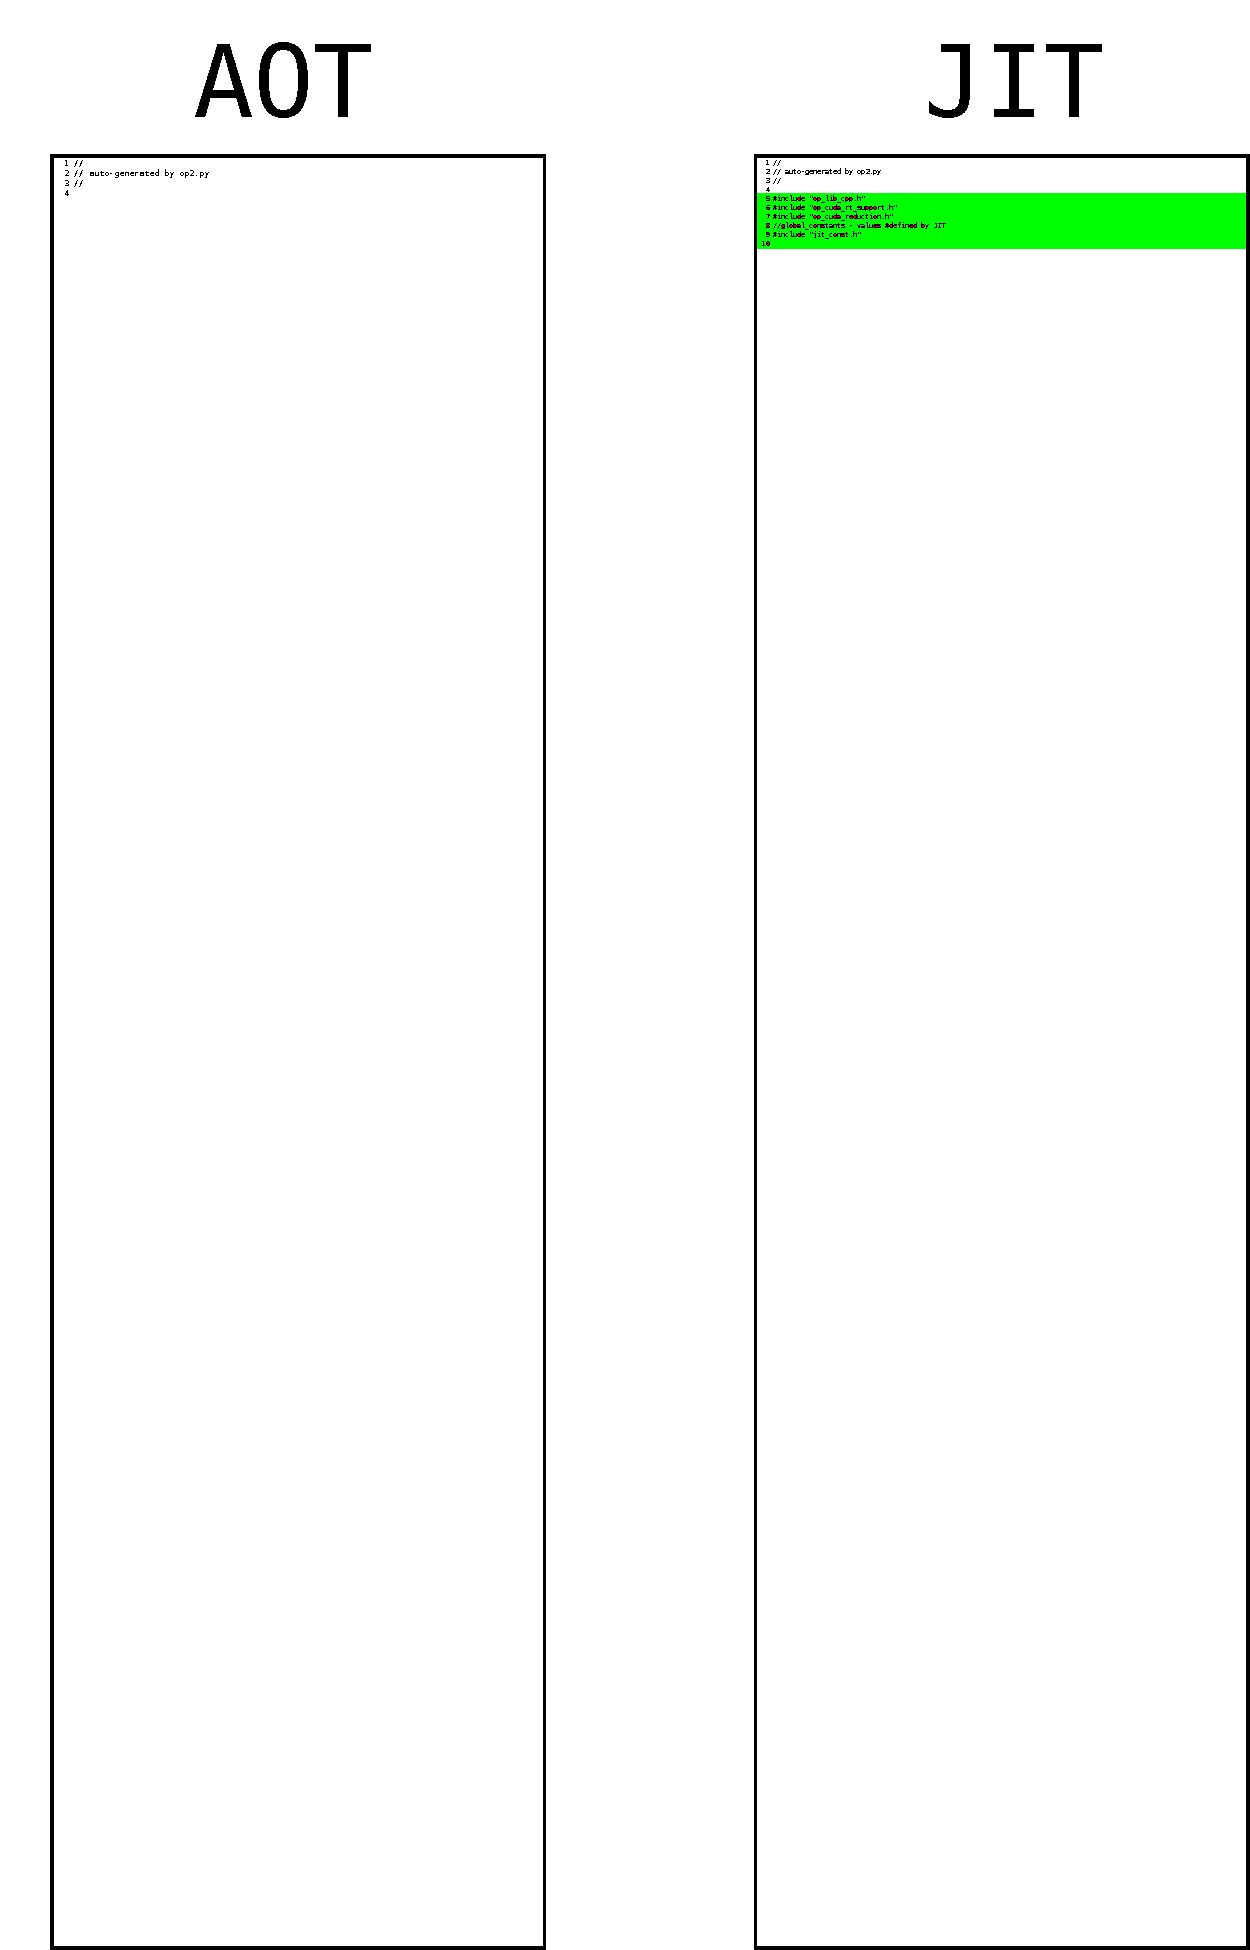
\includegraphics[width=.3\textwidth]{jit_include}
\end{wrapfigure}
\minititle{JIT includes}
The first part generated is simply the include directives required for the JIT compiled kernel. These are needed for JIT since they will be compiled individually, but aren't needed by the AOT kernel, as they will be included in the master kernels file:
\begin{lstlisting}[backgroundcolor = \color{green!20}, language=C]
 #include `op_lib_cpp.h'
 #include `op_cuda_rt_support.h'
 #include `op_cuda_reduction.h'

 //global_constants
 #include `jit_const.h'
\end{lstlisting}
The \verb|jit_const.h| file is also included, which will be generated at runtime (before the compiler is invoked) to contain a \verb|#define| for all constants, to be processed by the preprocessor.

\begin{wrapfigure}[12]{r}{.33\textwidth}
  \vspace{-2em}
  \centering
  \caption{User Function}
  \label{fig:usr_func}
  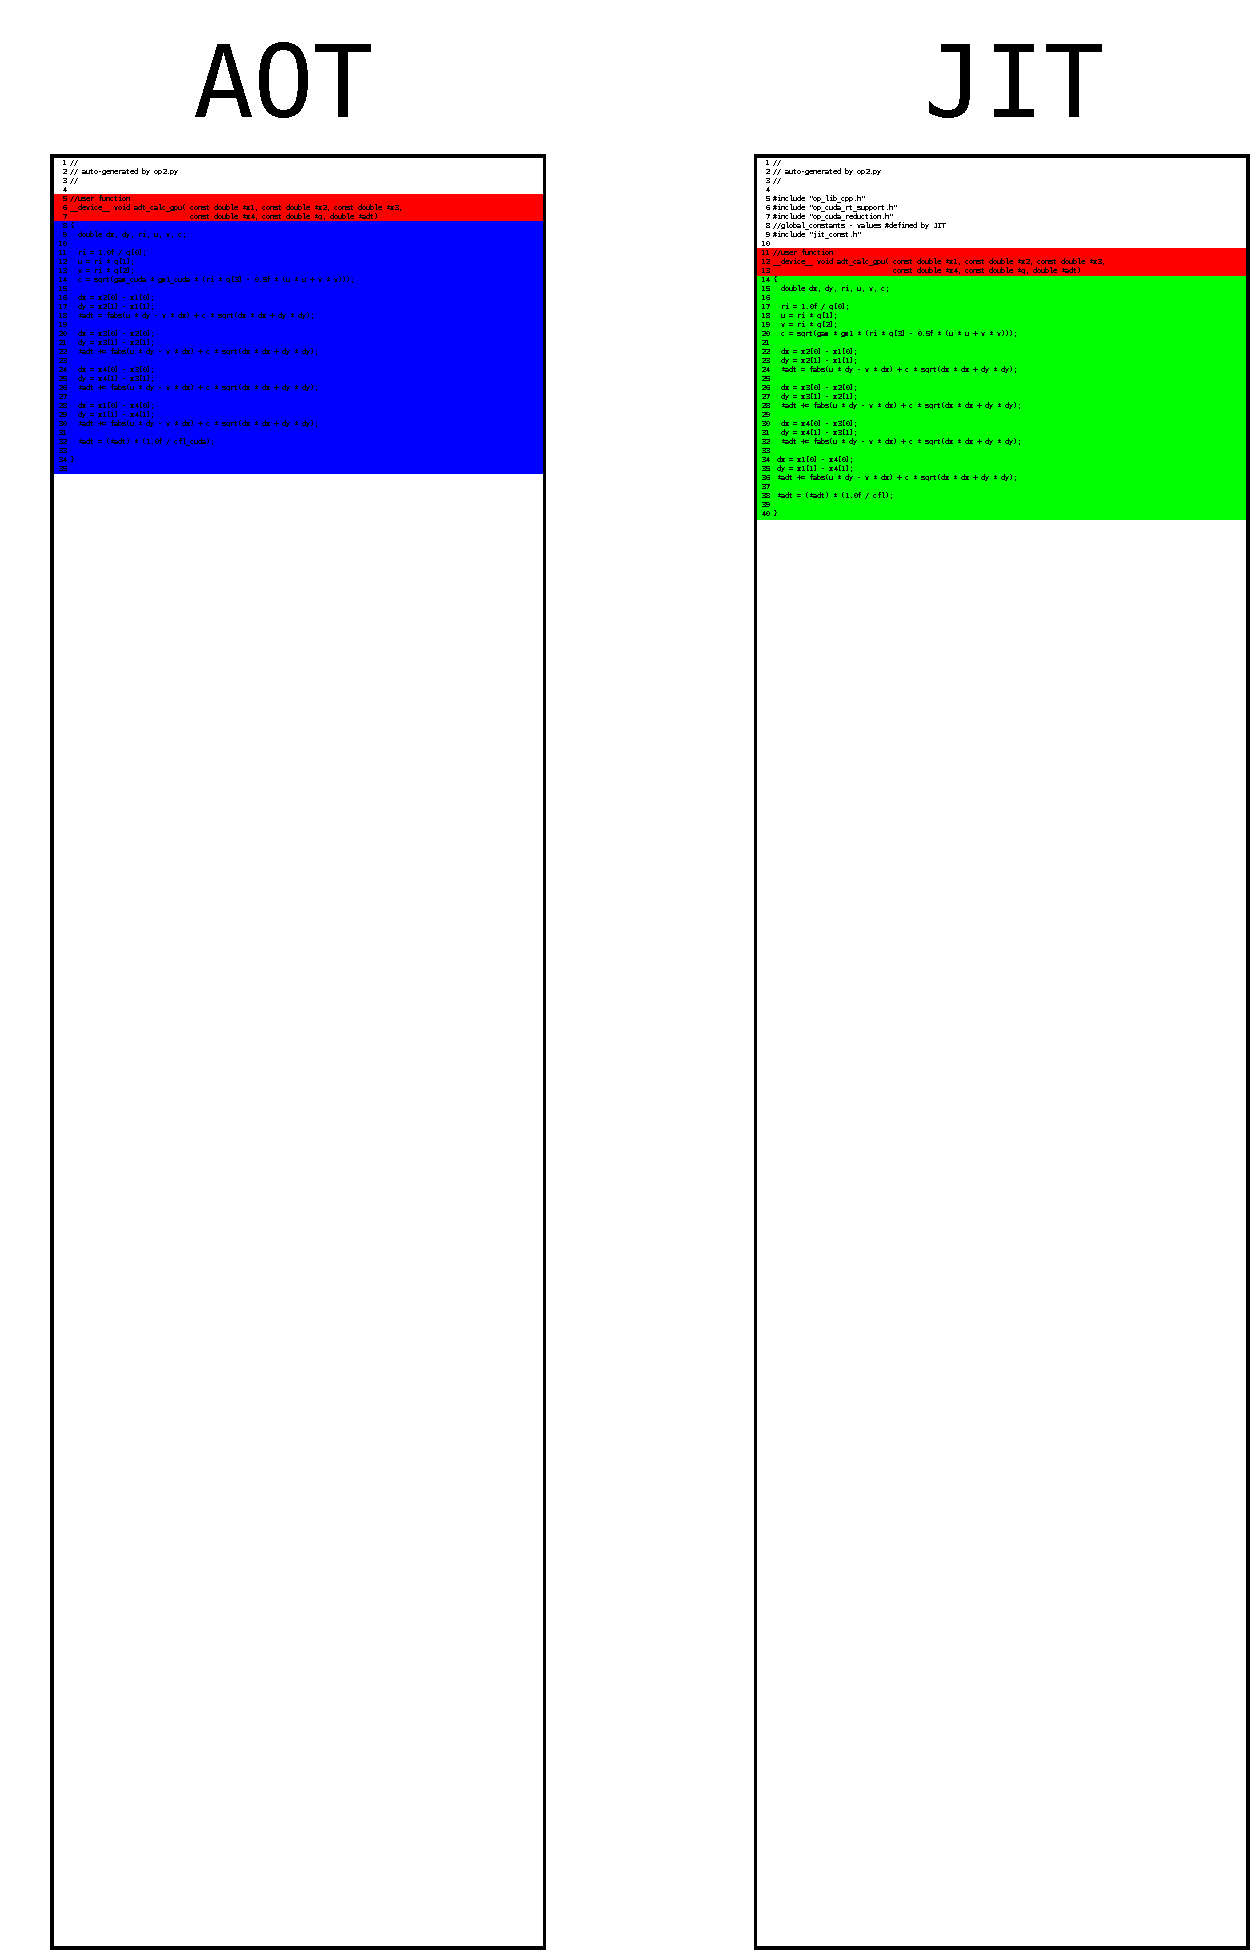
\includegraphics[width=.3\textwidth]{user_function}
\end{wrapfigure}
\minititle{User Function}
The User Function is the kernel operation specified by the user to be carried out on each iteration of the loop, so this function will run on the device (GPU) at least once for each set item. This function is given the signiture:
\codeline{__device__ void [name]_gpu( [args] )}{}
The \verb|__device__| descriptor is used so that it will be compiled for the GPU, and can only be called from other device code.
The kernel function found is checked to ensure it has the correct number of parameters, and, if requested, parameters are modified to utlise the struct of arrays layout.
\par
The User Function is where any runtime assertions need to be made in order to benefit from the additional computation once inputs are known. In this report the assertion applied is using a \verb|#define| for constants, so wherever the User Function references a constant it needs to be modifed.

\tinytitle{AOT}
In the Ahead-Of-Time kernel, only executed if JIT is not being used, the constant will need to read from the device's memory - having been copied there when it is defined constant. The copied version will have the identifier \verb|[id]_cuda| to prevent a name collision, so all constant in the AOT kernel must be replaced with this pattern.
\begin{lstlisting}[backgroundcolor = \color{lightgray!20}, language=Python]
for nc in range(0,len(consts)):
  varname = consts[nc]['name']
  aot_user_function = re.sub('\\b' + varname + '\\b',
                              varname + '_cuda',
                              aot_user_function)
\end{lstlisting}
\vspace{-1em}
\hspace*{\fill}\footnotesize{translator/c/python/jit/op2\_gen\_cuda\_jit.py [905-907]}

\tinytitle{JIT}
The JIT kernel is a little different: contants with a dimension of 1 (i.e. they contain only 1 value) can be left the unchanged, as the value will be defined under that same identifier. Multi-Value constants are slightly trickier - since values cannot be declared both \verb|__constant__| and defined as external using \verb|extern|\cite[p126]{guide}.
\par
The eventual solution to this challenge was in two parts. For each index \verb|N| of the constant array, a 1 dimensional constant would be defined with the name: \verb|op_const_[id]_[N]|. All references to the constant where the index is a literal number can be replaced with the new identifier:
\begin{lstlisting}[backgroundcolor = \color{lightgray!20}, language=Python]
for nc in range(0,len(consts)):
  varname = consts[nc]['name']
  if consts[nc]['dim'] != 1:
    jit_user_function = re.sub(`\\b' + varname + `\[([0-9]+)\]',
                               `op_const_' + varname + `_\g<1>',
                                jit_user_function)}
\end{lstlisting}
\vspace{-1em}
\hspace*{\fill}\footnotesize{translator/c/python/jit/op2\_gen\_cuda\_jit.py [931-934]}

If the constant is accessed using a variable, expression, or anything other than a literal number, this system won't work however. In this case, an array is defined at the top of the function (only if required) with the identifier \verb|op_const_[name]|, and the accesses are changed to match, so the access expression can remain and function as expected. This is only done where necessary, since allocating a new array can take time.
\begin{lstlisting}[backgroundcolor = \color{lightgray!20}, language=Python]
for nc in range(0,len(consts)):
  ...
  jit_user_function, numFound = re.subn(`\\b' + varname + `\[',
                                      `op_const_' + varname + `[',
                                       jit_user_function)
  #At least one expression access
  if (numFound > 0):
    if CPP:
      #Line start
      codeline = `__constant__ ' + consts[nc]['type'][1:-1] +
                 ` op_const_' + varname + `[' +
                  consts[nc]['dim'] + `] = {'
      #Add each value to line
      for i in range(0,int(consts[nc][`dim'])):
          codeline += `op_const_' + varname + `_' + str(i) + `, '
      codeline = codeline[:-2] + `};'

      jit_user_function = codeline+'\n\n'+jit_user_function
\end{lstlisting}
\vspace{-1em}
\hspace*{\fill}\footnotesize{translator/c/python/jit/op2\_gen\_cuda\_jit.py [931-944]}

\begin{wrapfigure}[17]{r}{.33\textwidth}
  \vspace{-1.2cm}
  \centering
  \caption{Kernel Function}
  \label{fig:krnl_func}
  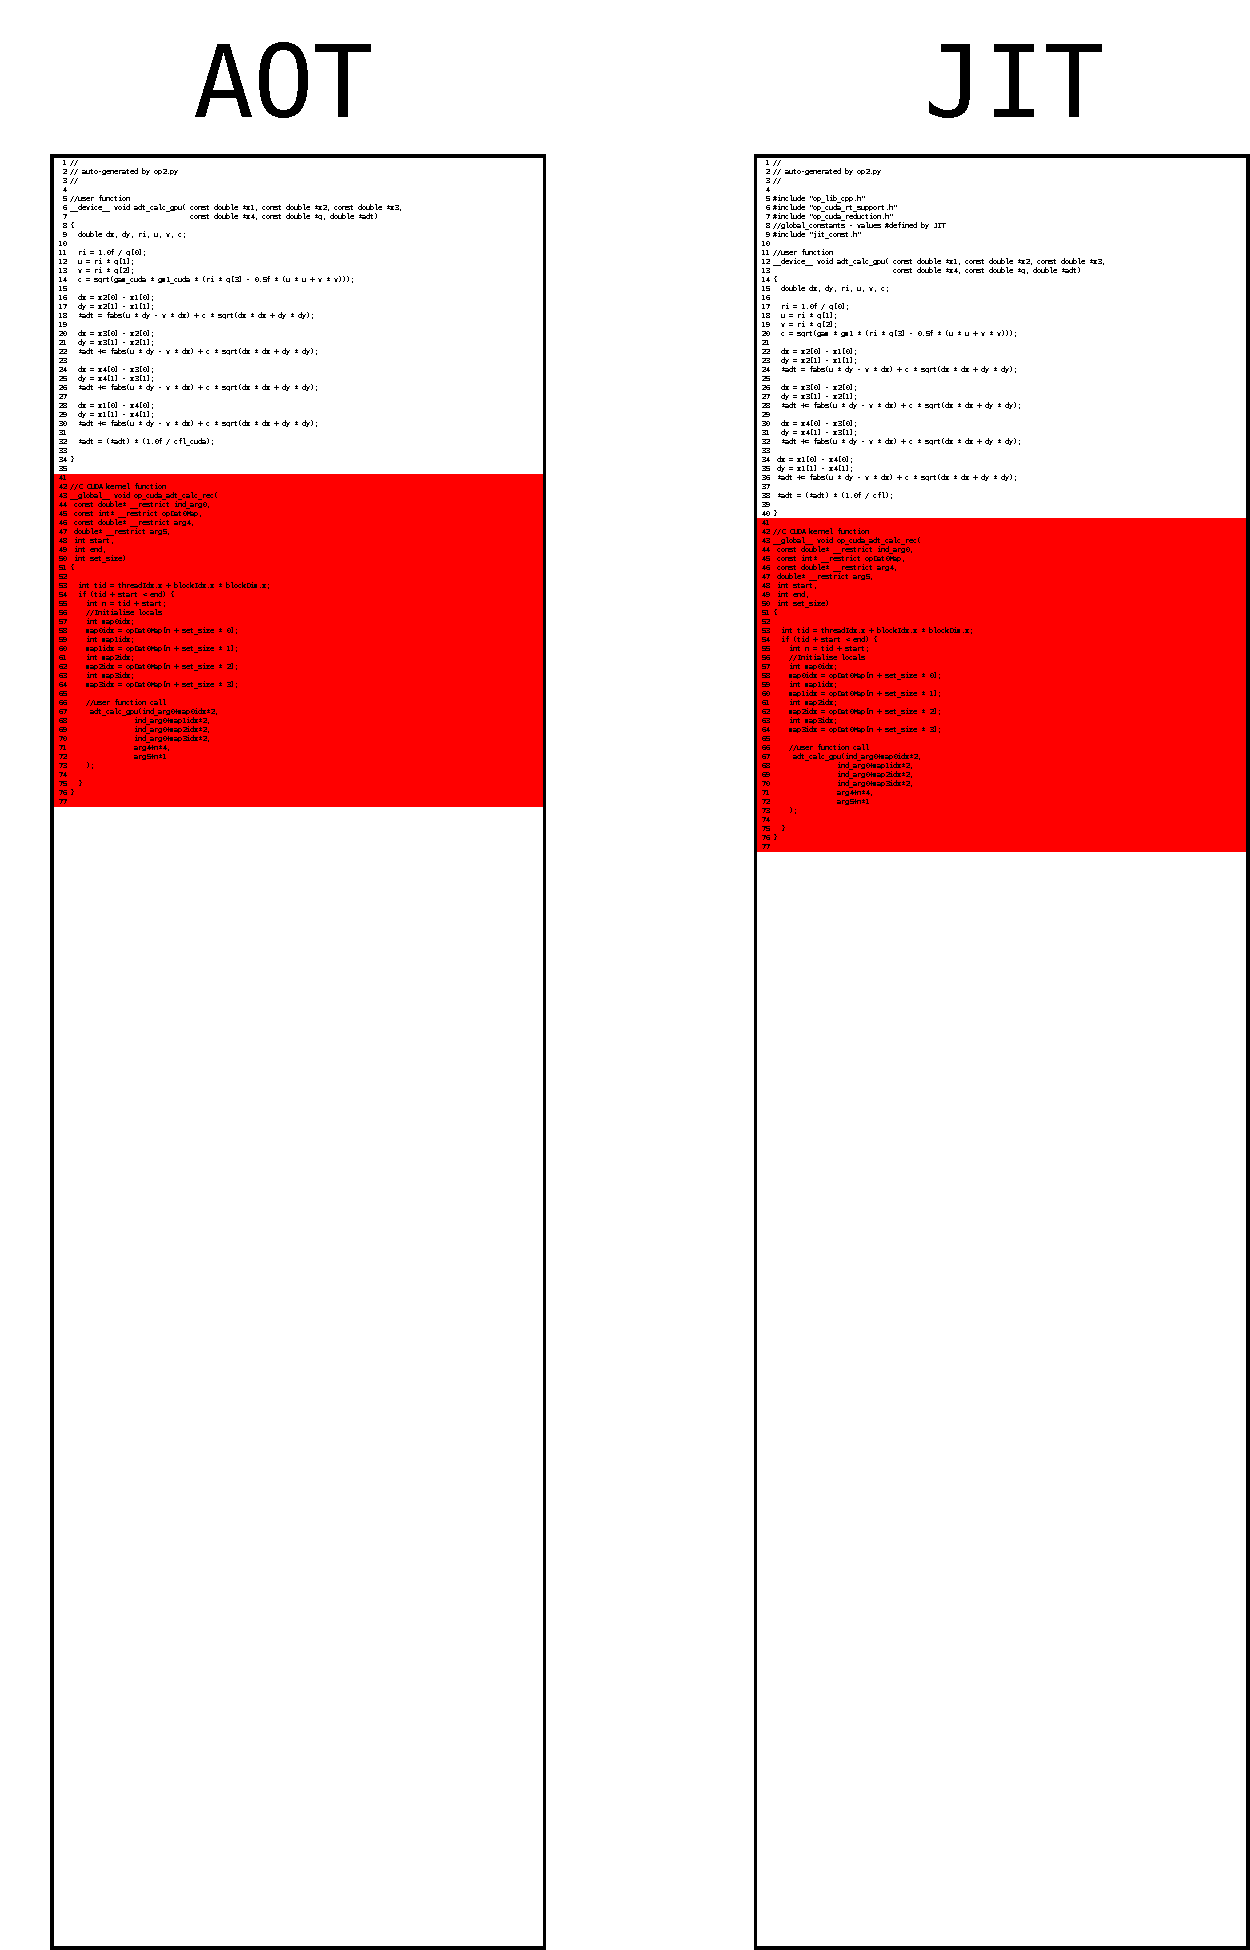
\includegraphics[width=.3\textwidth]{kernel_function}
\end{wrapfigure}
\minititle{Kernel Function}
From here onward, all code generated is based only on the kernel descriptor, and not the code that the user wrote for the body of the loop. The kernel function is the same in both files, and is executed on the GPU. It is declared \verb|__global__| so that is exectuted on the device, but can be called from host (CPU) code:
\codeline{__global__ void op_cuda_'+name+'( [args] )}{}
The function arguments depend on whether any of the arguments are optional, and whether the loop uses indirection - accessing a set using an index which is the value in another set. OP2 enforces that the operands in the set operations are referenced through at most a single level of indirection \cite[p4]{manual}.
\par
The function body also depends on whether there is indirection, as the indicies need to be retrieved from the inner map. A call is made to the user function generated above, then any reductions on arguments needs to be done. The supported reductions are: sum, maximum, and minimum\cite[p11]{manual}.

\begin{wrapfigure}[8]{r}{.33\textwidth}
  \vspace{-1.5cm}
  \centering
  \caption{Host Function}
  \label{fig:host_func}
  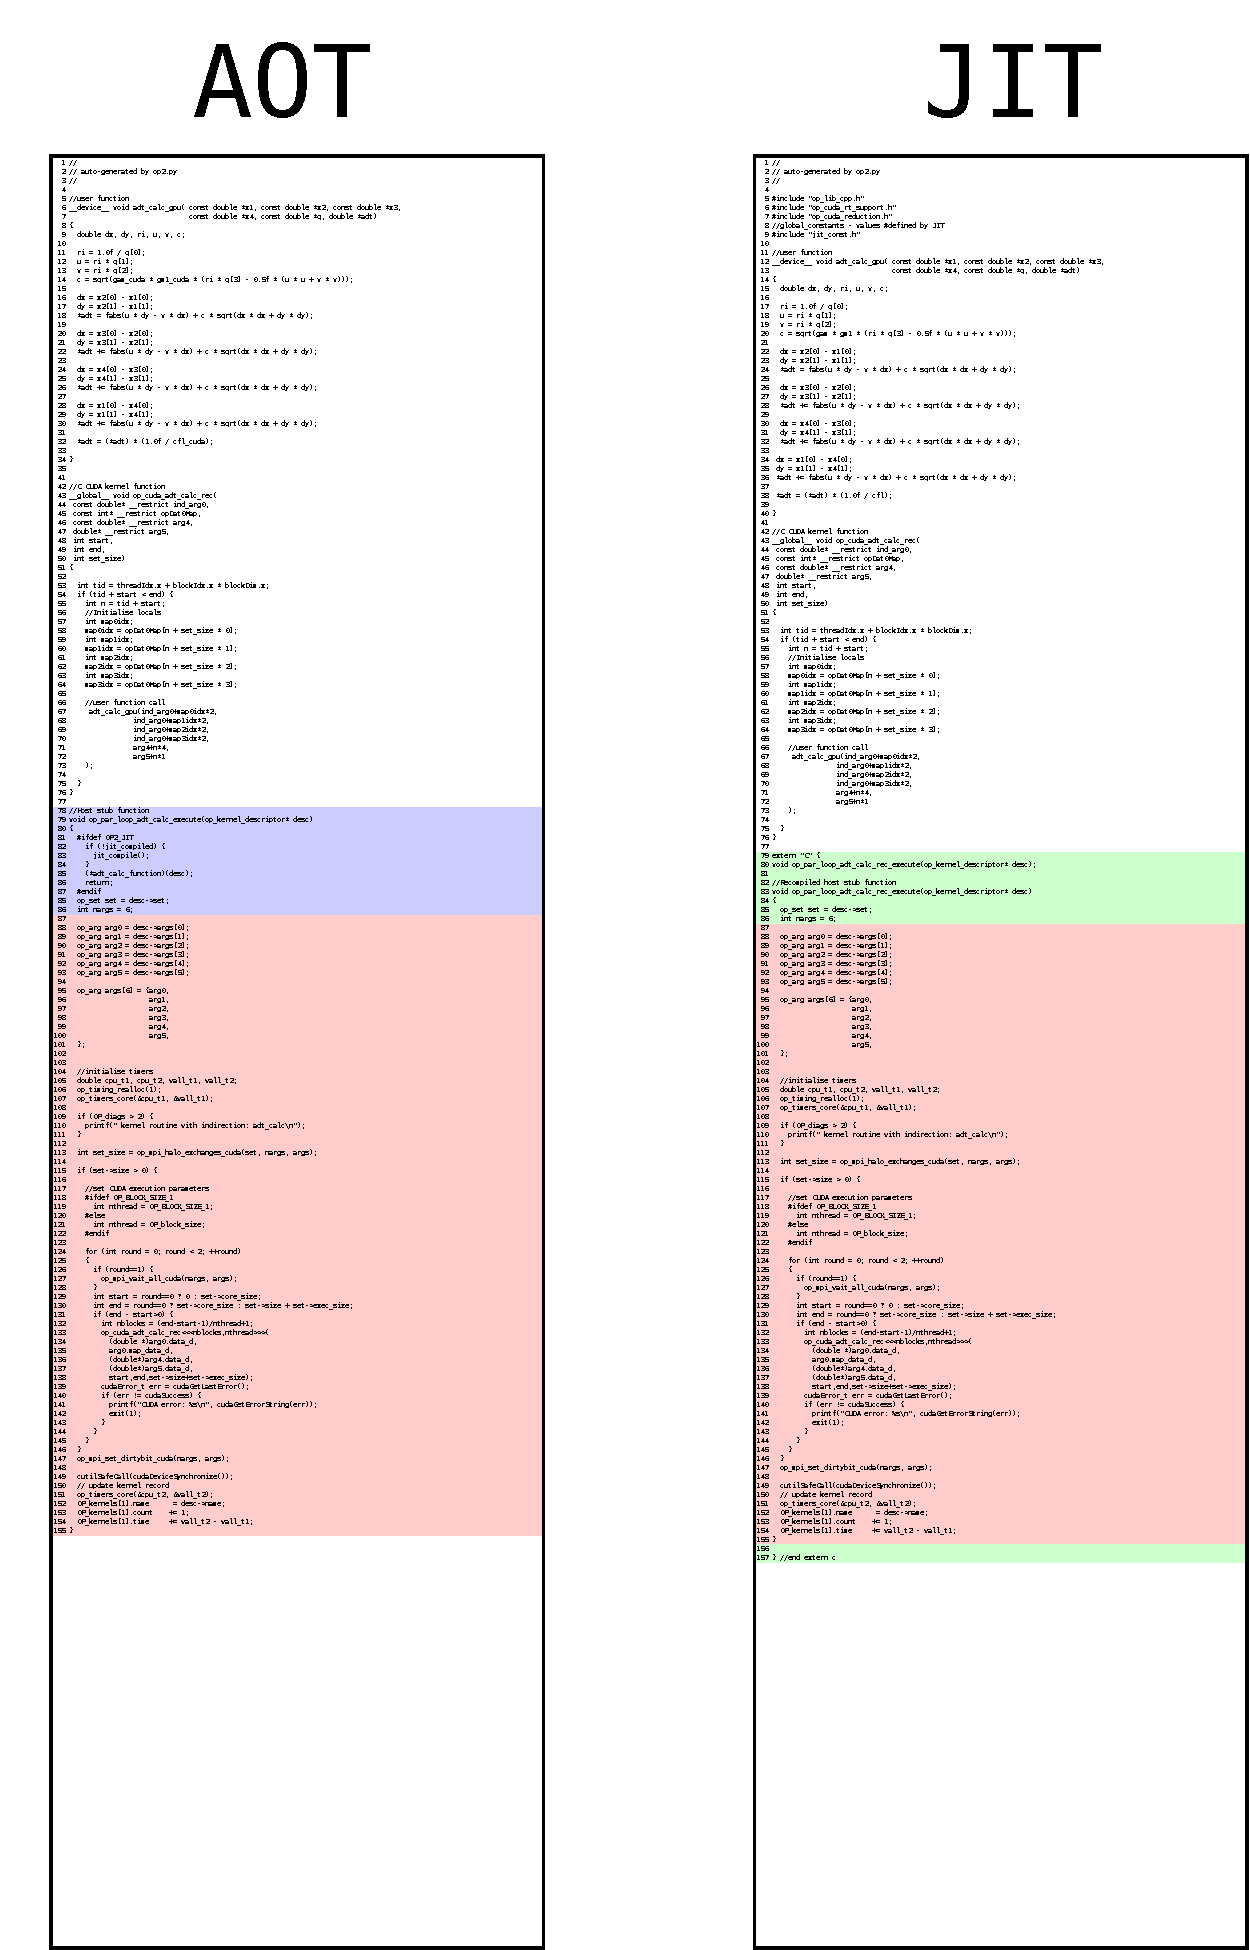
\includegraphics[width=.3\textwidth]{host_function}
\end{wrapfigure}
\minititle{Host Function}
The purpose of the host function is to bridge the gap between the host and the device. It is CPU code, so runs on the host, but contains the CUDA call to the kernel function which will run on the GPU. While the function body is the same for both AOT and JIT: setting up arguments, timers, and block and thread sizes for the CUDA call; the function head differs, as shown in Figure \ref{fig:host_func}.
\vspace{\parskip}

\tinytitle{AOT}
In the Ahead-Of-Time kernel file, the C code generated for the head of the host function is as follows:

\begin{lstlisting}[linewidth = \textwidth, framesep=0pt, language=C, linebackgroundcolor={\ifnum\value{lstnumber}=14\color{red!20} \else \color{blue!20} \fi}]
 //Host stub function
 void op_par_loop_[name]_execute(op_kernel_descriptor* desc)
 {
   #ifdef OP2_JIT
     if (!jit_compiled) {
       jit_compile();
     }
     (*[name]_function)(desc);
     return;
   #endif

   op_set set = desc->set;
   int nargs = 6;
   ... //Identical Section
 }
\end{lstlisting}
\vspace{-1em}
The function name is \verb|op_par_loop_[name]_execute| because a pointer to this function will be queued by the lazy execution system mentioned previously in this Section, so this function actually executes the loop, whenever the lazy execution system should decide it needs to be executed. The decision of when to call the loop is outside the scope of this project, and currently a loop is simply called immediately after it is queued.
\par At the top of the function a decision is made as to whether JIT should be used, based on whether \verb|OP2_JIT| has been defined. This allows JIT to be turned on and off through the used the compiler argument \verb|-DOP2_JIT|. If JIT is enabled, then the compiler is invoked (if it hasn't been already), and the pointer to the newly compiler version of the function is executed instead.
\par
If JIT is not enabled, this code will be ignored by the compiler, so the process will continue into the AOT host function, which causes it to stay whithin the AOT kernel file and never execute any code from the JIT file.

\tinytitle{JIT}
Contrasting this with the code generated for the JIT kernel file:

\begin{lstlisting}[linewidth = \textwidth, framesep=0pt, linebackgroundcolor={\ifnum\value{lstnumber}=9\color{red!20} \else \color{green!20} \fi}]
 extern "C" {
 void op_par_loop_[name]_rec_execute(op_kernel_descriptor* desc);

 //Recompiled host stub function
 void op_par_loop_[name]_rec_execute(op_kernel_descriptor* desc)
 {
   op_set set = desc->set;
   int nargs = 6;
   ... //Identical Section
 }

 } //end extern c
\end{lstlisting}
\vspace{-1em}

Firstly, since this function needs to be linked to the exisiting code as part of a dynamically loaded library, it is placed inside an \verb|extern "C"| scope, to ensure C linkage, and prevent the compiler from "mangling" the name. Following that, the function, which is named\\
\verb|op_par_loop_[name]_rec_execute| ("rec" short for recompiled), will come to reside in the address of the \verb|[name]_function| function pointer.
\par
It will be executed after the runtime compiler has been invoked, as the replacement JIT-compiled host function, and make calls to the kernel and user functions in the same file as iteself, rather than those in the AOT file - allowing the optimisations made to be used.

\minititle{Loop Function}
The last section to be generated in the kernel files is the Loop Function, which is the entry point for the parallel loop:
\codeline{op_par_loop_[name](char* name, op_set set, [args]... )}{}

\begin{wrapfigure}[12]{r}{.33\textwidth}
  \vspace{-3em}
  \centering
  \caption{Loop Function}
  \label{fig:loop_func}
  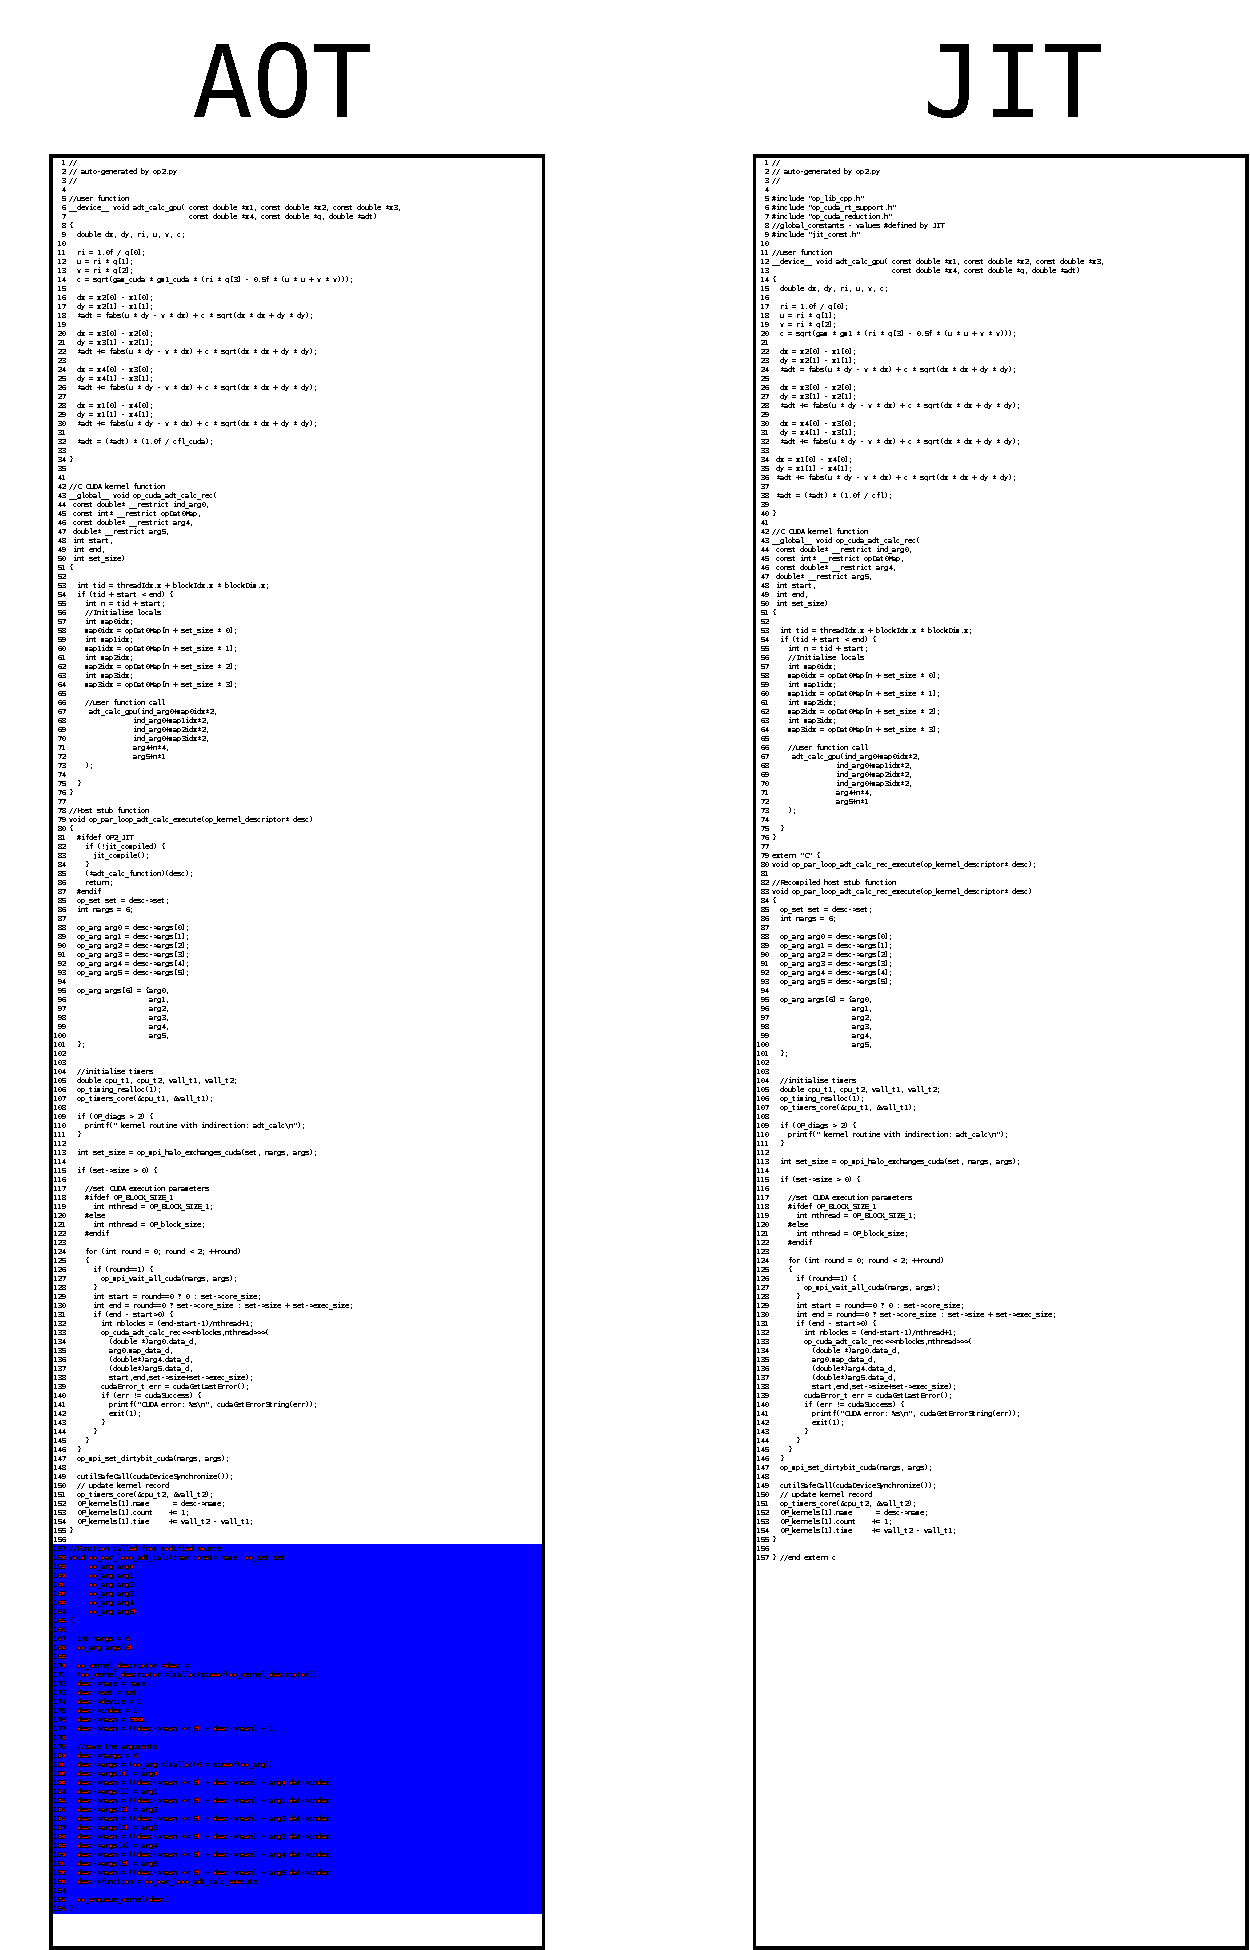
\includegraphics[width=.3\textwidth]{loop_function}
\end{wrapfigure}
The application file will be modified by \verb|op2.py| to contain an declaration for this function marked \verb|extern|, to be linked againt this definition. Only the AOT kernel requires this, as previously mentioned the JIT host function acts as its entry point (Figure \ref{fig:loop_func}).
\\
The purpose of this function is to generate the kernel descriptor, then make a call to:
\codeline{void op_enqueue_kernel(op_kernel_descriptor *desc)}{op2/c/src/core/op\_lazy.cpp [71-89]}

\noindent As previously mentioned, the kernel descriptor and enqueue function were part of the work done to enable lazy execution in OP2, and not created as part of this project.

\vspace{2em}

\begin{wrapfigure}[13]{l}{.4\textwidth}
  \vspace{-2em}
  \centering
  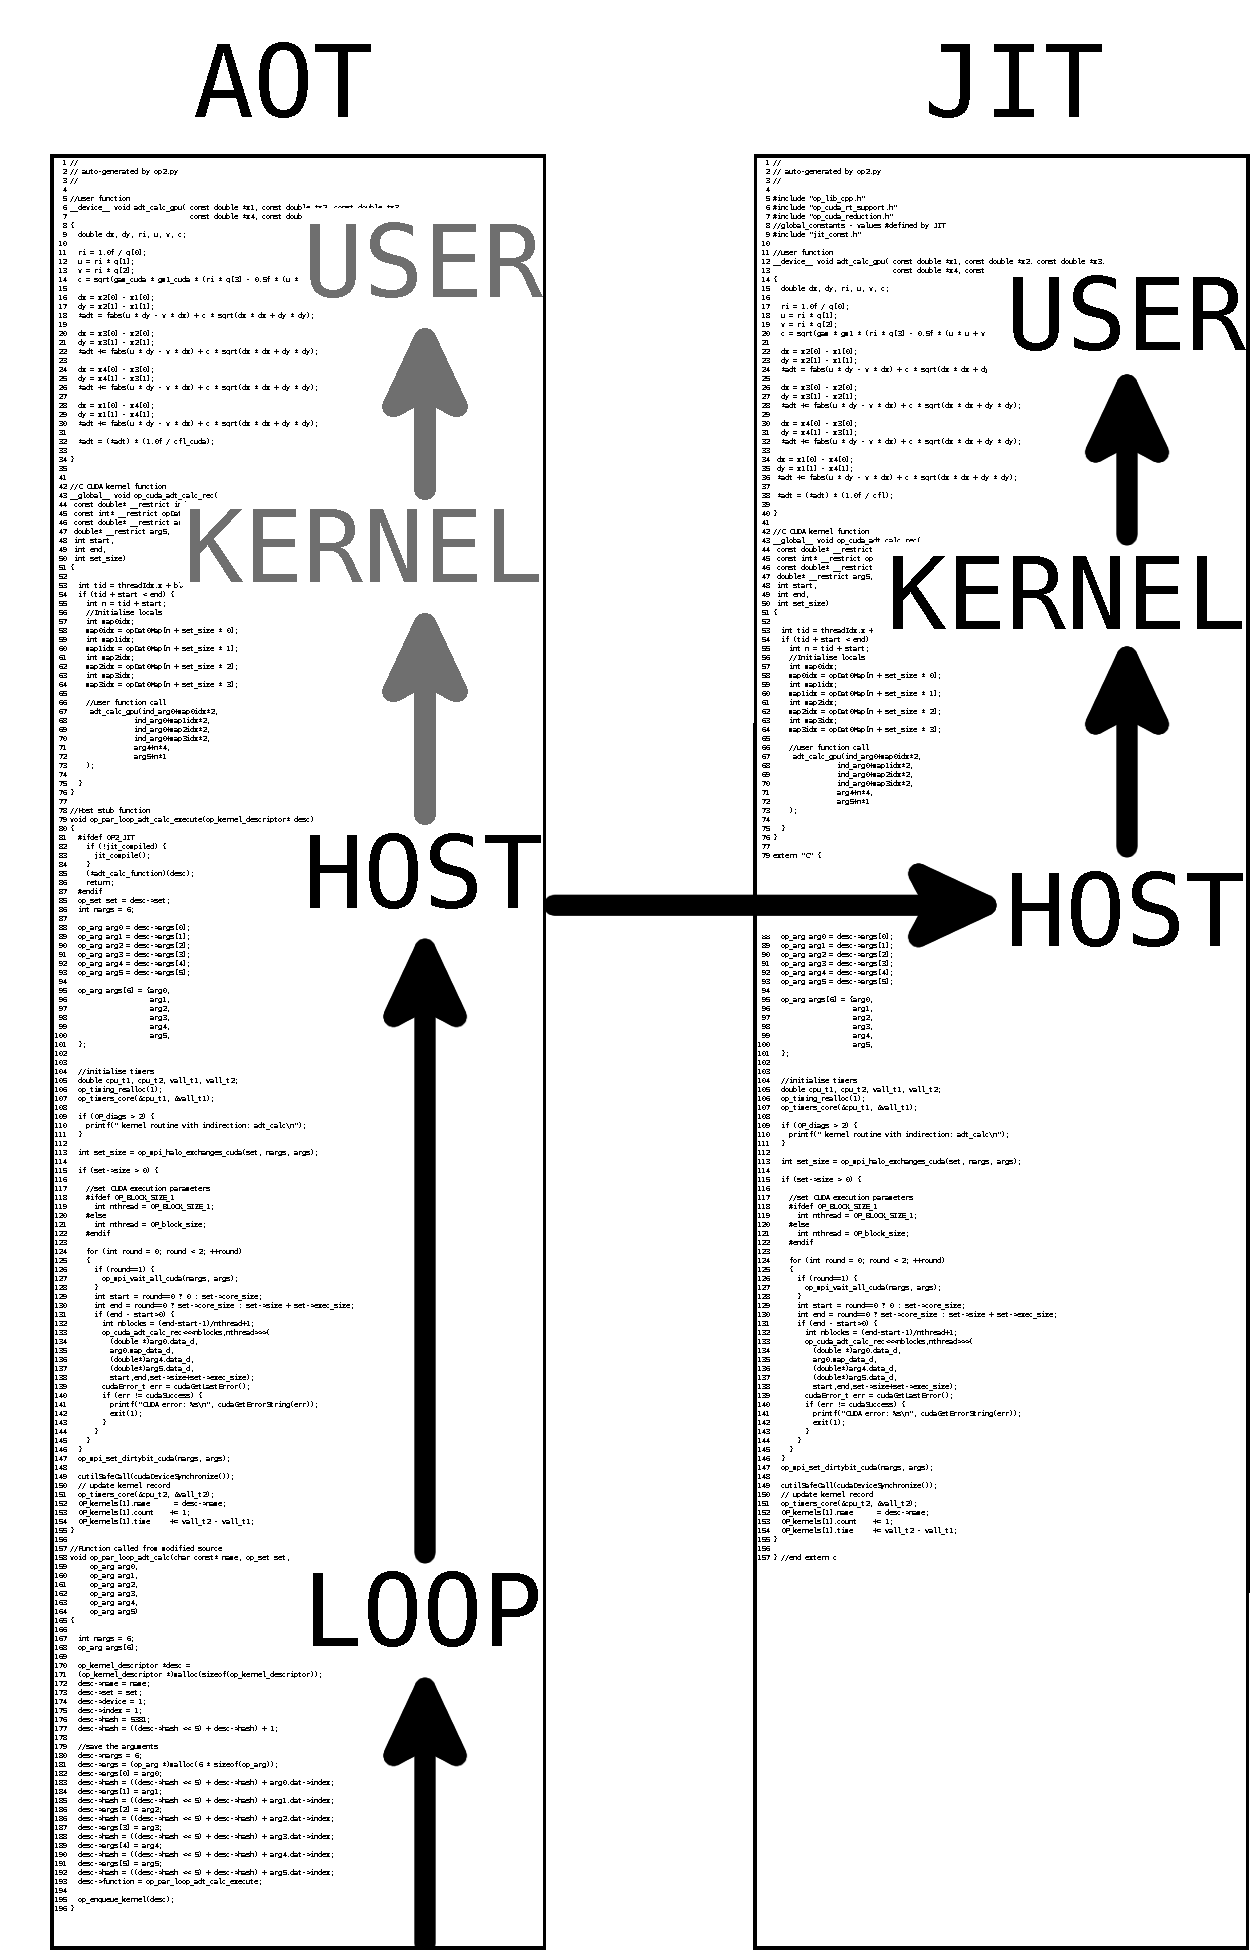
\includegraphics[width=.39\textwidth]{krnl_flow}
  \caption{Kernel Flow}
  \label{fig:krnl_flow}
\end{wrapfigure}

\tinytitle{Summary}
\label{impl_summary}

To recap, the AOT and JIT kernel files are generated for each parallel loop, to be executed when that loop is invoked in the application file. Figure \ref{fig:krnl_flow} has been included to make clear the data flow through the two files: starting in the Loop Function, which calls the AOT Host Function, where either the re-compiled version is invoked, or the original version is used if JIT is not enabled at compile time.

The \verb|jit_compile()| function has not yet been defined, but this will be covered in the next section on the master kernels file.
\clearpage
\subsubsection{Master Kernels File}
\label{sss:mkf}
The Master Kernels File: \verb|cuda/[application]_kernels.cu| is the last file to be generated, once the kernels for each parallel loop have been completed. It ties up most of the remaining loose ends, as it contains shared functions for invoking the runtime compiler, and declaring constants. It also contains \verb|#include| statements for each of the AOT kernel files, so that the application file can be linked against this file only at compile-time, and the linker will be able to find definitions for all the functions declared extern. The Makefile and compile process will be covered further in Section TODO.
\par
At the top, the master kernels file includes the requried OP2 library files. It then defines a CUDA constant for each constant the user has defined, generated using the following python code:
\begin{lstlisting}[backgroundcolor = \color{lightgray!20}, language=Python]
for nc in range (0,len(consts)):
  if consts[nc]['dim']==1:
    # __constant__ [type] [name]_cuda;
    code('__constant__ ' + consts[nc]['type'][1:-1] + ' ' +
          consts[nc]['name'] + '_cuda;')
  else:
    if consts[nc]['dim'] > 0:
      num = str(consts[nc]['dim'])
    else:
      num = 'MAX_CONST_SIZE'

    # __constant__ [type] [name]_cuda[ [dim] ];
    code('__constant__ ' + consts[nc]['type'][1:-1] + ' ' +
          consts[nc]['name'] + '_cuda' + '['+num+'];')
\end{lstlisting}
\vspace{-1em}
\hspace*{\fill}\footnotesize{translator/c/python/jit/op2\_gen\_cuda\_jit.py [974-985]
\\
Following this, the file contains definitions for two functions. The first is \verb|op_decl_const_char|, which will be called from the application file to declare a constant identifier and value; and the second is \verb|jit_compile| which will invoke the runtime compiler, load the generated DLL and create a function pointer for each re-compiled loop.

\minititle{op\_decl\_const\_char}
This function is an OP2 library function which allows users to declare a value that will not change over the course of execution. It has the following signature, defined by the OP2 API\cite[p9]{manual}:
\codeline{void op_decl_const_char(int dim, char const *type, int size,
                                  char *dat, char const *name)}{}
 Two versions of the function are generated, one for AOT and one for JIT. The two functions are wrapped with pre-processor conditionals, so that only one of them will be visible to the compiler. As before, \verb|OP2_JIT| being defined is the test, so the JIT functionality can be enabled or disabled.
\par
The AOT version of the function copies the value passed to it to the corresponding device constant using:
\codeline{cudaMemcpyToSymbol(const void* symbol, const void* src, size_t count)}{}
The copy default direction for this function is from host memory to device memory.
\par
The JIT version instead invokes the internal library function:
\codeline{void op_lazy_const(int dim, char const *type, int typeSize, char *data,
                        char const *name)}{op2/c/src/core/op\_lazy.cpp [100-101]}
Which maintains a de-duplicated list of constants, so that once they all have been declared the header file defining their values can be generated. As can be seen in the generated C code below, constants containing more than one value are declared as single values due to the issues with \verb|extern __constant__| values described in Section \ref{ss:krnl_files} (2. User Function).
\begin{lstlisting}[linewidth = \textwidth, framesep=0pt]
void op_decl_const_char(int dim, char const *type,
                        int size, char *dat,
                        char const *name)
{
  if (dim == 1) {
    op_lazy_const(dim, type, size, dat, name);
  }
  else {
    for (int d = 0; d < dim; ++d)
    {
      char name2[32];
      sprintf(name2, "op_const_%s_%d\0", name, d);
      op_lazy_const(1, type, size, dat+(d*size), name2);
    }
  }
}
\end{lstlisting}
\vspace{-1em}
\hspace*{\fill}\footnotesize{generated by translator/c/python/jit/op2\_gen\_cuda\_jit.py [1028-1046]}

\minititle{jit\_compile}
The other function generated is the \verb|jit_compile| function, which is responsible for the actual recompilation of the JIT kernels, and making their functions available to the binary. It also uses the same timing library functions which gather data on the time spent in each parallel loop to determine how long the binary spends re-compiling, as this is important for performance measuring later.
\par
The compiler arguments, library paths, and other required parameters are in this implementation handled by a make file which would need to be generated by the user. The contents of the makefile will be covered in the next section.
\par
As can be seen below, the executable makes a system call to initiate a make command, and stores the result in a log file. If the compilation fails, an error message is printed, and the program exits early.
\begin{lstlisting}[linewidth = \textwidth, framesep=0pt]
if (op_is_root()) {
  if (system("make -j [application]_cuda_rec &> jit_compile.log"))
  {
    // 0 indicated success
    printf("Error: JIT compile failed. \n
            - see jit_compile.log for details\n");
    exit(1);
  }
}
\end{lstlisting}
\vspace{-1em}
\hspace*{\fill}\footnotesize{generated by translator/c/python/jit/op2\_gen\_cuda\_jit.py [1071-1077]}

It is expected that the make file will generate a shared object file named \verb|cuda/airfoil_kernel_rec.so|. If this file does not exist the binary exits with an error, otherwise the recompiled function for each parallel loop is dynamically loaded using:
\codeline{void *dlsym(void *restrict handle, const char *restrict name);}{dlfcn.h}
The function \verb|op_par_loop_[name]_rec_execute| loaded, with the address stored in a void pointer with identifer \verb|[name]_function|. We have seen this pointer before in Section \ref{ss:krnl_files} (4. Host Function).
\par
Once this has been done for all loops, the wall clock time since the start of the \verb|jit_compile| function is printed to the terminal.

\subsection{Makefile}
This implementation relies on GNU Make\cite{make} to determine which compiler should be used, which parameters should be passed, and other options. There are a number of libraries required to build an OP2 binary, as covered in Appendix \ref{app:getStart}, so only the recompilation target will be discussed here.
\par
The binary expects there to be a Makefile in the directory it executes in, with a target: \verb|[application]_cuda_rec| in order to work correctly. This is the target which will be compiled at runtime. As mentioned in the previous section, the result of making this target needs to be a a shared object file named \verb|cuda/airfoil_kernel_rec.so|, which contains the recompiled loop functions.
\par
The library object is produced by compiling each of the kernels individually, using the NVidia compiler \verb|nvcc| from the NVidia CUDA Toolkit\cite{nvcc,toolkit} as the code contains CUDA, then linking them into a single object. It is necessary that the compiler flags include \verb|--compiler-options -fPIC|. This passes a list of arguments to the underlying compiler, since nvcc only handles the CUDA code, and passes all host code compilation on to a C compiler. The argument to be passed down is \verb|-fPIC|, to generate Position Independant Code, to allow the library function to execute correctly, regardless of the address at which it is loaded in memory.
\subsubsection{Optional Functionality}
By default, the JIT compilation functionality is enabled in the Makefile by setting the value of \verb|$JIT| to \verb|TRUE|. However, if the variable is set to anything else in the parameters of the make command, JIT will be disabled in the resulting executable. This is done with the following lines:
\begin{lstlisting}[linewidth = \textwidth, framesep=0pt]
ifeq ($(JIT), TRUE)
	CCFLAGS    := $(CCFLAGS) -DOP2_JIT
	NVCCFLAGS  := $(NVCCFLAGS) -DOP2_JIT
	SUFFIX     := _jit
endif
\end{lstlisting}
Which adds a parameter to the C and CUDA compilers to define \verb|OP2_JIT| for the preprocessor, and appends "\_jit" to the name of the executable generated.
\par
The target \verb|cuda/airfoil_kernels_cu.o| is also declared PHONY, so that it is always recompiled even if the file already exists, otherwise this make flag would not function correctly, and a JIT enabled version of this file may be used when the user intended to recompile it with JIT disabled.
